\documentclass[11pt,a4paper]{article}

\usepackage[T1]{fontenc}
\usepackage[margin=2.3cm]{geometry}
\usepackage{amsmath,amssymb}
\usepackage{booktabs}
\usepackage{array}
\usepackage{enumitem}
\usepackage{graphicx}
\usepackage{tikz}
\usetikzlibrary{arrows.meta,positioning,patterns}
\usepackage[most]{tcolorbox}
\usepackage[hidelinks]{hyperref}
\usepackage{parskip}

\setlist{itemsep=2pt,topsep=3pt}
\renewcommand{\arraystretch}{1.25}

% grey boxes only
\newtcolorbox{keybox}[1][]{colback=gray!10,colframe=black!60,boxrule=0.5pt,arc=2pt,left=6pt,right=6pt,top=4pt,bottom=4pt,#1}
\newtcolorbox{saybox}[1][]{colback=white,colframe=black!40,boxrule=0.5pt,arc=2pt,left=6pt,right=6pt,top=4pt,bottom=4pt,fonttitle=\bfseries,title={#1}}

\title{\textbf{Midterm Report: Explanation Guide}\\[4pt]
\large Change-Characteristic-Aware Window Selection for Unsupervised Concept Drift Detection in Real-Time Text Streams}
\author{Group guide for the class discussion\\Course: Big Data Technologies}
\date{}

\begin{document}
\maketitle

\begin{keybox}
\textbf{How to use this guide.} This guide helps us explain and justify our midterm report (\texttt{Midterm\_Report\_V3}) in class. It follows the order of a good talk: the problem, the base paper, the gap, our idea, the figures, the plan, and likely questions. Simple words are used on purpose. Part~\ref{sec:oneminute} is a one-minute summary and Part~\ref{sec:qa} lists questions the faculty may ask.
\end{keybox}

\tableofcontents
\newpage

%====================================================================
\section{The Project in One Minute}
\label{sec:oneminute}

\begin{saybox}{What we can say in one minute}
Text keeps arriving all the time, for example news, posts and reviews. Over time the topics and words change. This is called \emph{concept drift}. When it happens, a model trained on old text becomes less accurate. So a real-time system must notice the change quickly.

Most detectors need the correct label of every new document, but in real life labels are late or missing. Our base paper, \textbf{ADWIN-U}, detects drift \emph{without labels}. It keeps a window of recent data and cuts away the old part when a change appears.

We found one weak point. ADWIN-U always makes the same decision: either it cuts the whole old part or it does nothing. It does not look at \emph{how strong} or \emph{how long} the change is. We propose a small rule that adds a \textbf{hold} state and a \textbf{partial cut}. We will test it on text streams, where ADWIN-U was never tested.
\end{saybox}

\paragraph{Very short version (one sentence).}
We improve how an unsupervised drift detector decides to cut its window, and we test it on text streams.

%====================================================================
\section{Background: What Do We Need to Know First?}

\subsection{What is a data stream?}
A data stream is data that keeps arriving one item at a time, and it never ends. We cannot store everything and read it again. So each item should be processed once and quickly. Examples are news feeds, social media posts and product reviews.

\subsection{What is concept drift?}
Concept drift means the data changes over time. For example, a news classifier was trained before a big event. After the event, new subjects and new words appear. The old model does not understand them well, so its accuracy drops.

In the report we write this as
\[
P_t(X,Y)\neq P_{t+\Delta}(X,Y).
\]
\textbf{Meaning in simple words:} $X$ is the document (its features) and $Y$ is its label. $P_t(X,Y)$ is ``how the data looks at time $t$''. The formula says: the data at time $t$ looks different from the data a little later at time $t+\Delta$. If it does, drift has happened.

\subsection{Types of drift}
The report uses four common types (Section~II-A).

\begin{center}
\begin{tabular}{@{}>{\bfseries}p{2.6cm}p{6.5cm}p{4.5cm}@{}}
\toprule
Type & What happens & Easy example \\
\midrule
Abrupt & One concept is replaced by another at a single point. & News suddenly turns to a new event. \\
Gradual & Old and new concepts are mixed for a while. & Slowly more posts talk about a new topic. \\
Incremental & The data moves a little at a time. & Word usage slowly shifts. \\
Recurring & An old concept comes back. & Seasonal topics like holidays. \\
\bottomrule
\end{tabular}
\end{center}

\subsection{Virtual drift and real drift}
\emph{Real drift} changes the link between the document and its label. \emph{Virtual drift} changes only how the documents look, $P(X)$. A detector that uses no labels can only see virtual drift. This is fine for us, because a change in the documents is a good early warning.

\subsection{Why labels are a problem}
Classic detectors such as DDM and ADWIN watch the \emph{error rate} of a classifier. To compute the error they need the true label after every prediction. For text, labels arrive late or never, because a person must read and label each document. So we need a detector that works \textbf{without labels}. This is called \emph{unsupervised} drift detection.

\subsection{What is a window and why is its size important?}
Many detectors compare a \emph{window} of recent data with a window of older data. If the two are very different, something has changed.
\begin{itemize}
  \item A \textbf{short} window reacts fast, but it is easily fooled by normal noise (false alarms).
  \item A \textbf{long} window is stable, but it reacts slowly (late alarms).
\end{itemize}
Also, the best size depends on the drift. A gradual or small change needs more data to be seen than an abrupt one. So a fixed window size is never best for every case. This is the main problem we work on.

%====================================================================
\section{Big Data Characteristics in Our Project}

Our faculty asked us to cover at least three characteristics of big data. We cover three: \textbf{Velocity, Variety and Veracity}. We do \emph{not} claim Volume.

\begin{center}
\begin{tabular}{@{}>{\bfseries}p{2.9cm}p{5cm}p{6cm}@{}}
\toprule
Characteristic & Why it applies to text streams & How our method handles it \\
\midrule
Velocity & Documents arrive all the time and must be processed in one pass. & The window is compact (bucketed) and is updated in almost constant time, so we can keep up with the stream. We will also measure latency and throughput. \\
Variety & Text is unstructured and differs in topic, source and style. & We turn text into sentence embeddings (fixed-length vectors), so the same detector works for news, newsgroup posts and reviews. \\
Veracity & Labels are missing and the true drift points are usually unknown, so the data is uncertain. & The method uses no labels. The hold state means it does not act on one weak signal, which reduces false alarms. \\
\bottomrule
\end{tabular}
\end{center}

\begin{keybox}
\textbf{Be careful with Variety.} We use only text. So our variety means different topics, genres and writing styles. We should \emph{not} say ``many data types''. If asked about Volume, we can say: ``We do not claim Volume. Our focus is velocity, variety and veracity.''
\end{keybox}

%====================================================================
\section{Our Base Paper}

\subsection{Which paper is it?}
Our base paper is \textbf{ADWIN-U}:

\begin{quote}
D.~N. Assis and V.~M.~A. Souza, ``ADWIN-U: Adaptive windowing for unsupervised drift detection on data streams,'' \emph{Knowledge and Information Systems}, vol.~67, no.~11, 2025.
\end{quote}

It is a journal paper. It builds on the older \textbf{ADWIN} method by Bifet and Gavald\`a (SIAM Data Mining Conference, 2007).

\subsection{What is ADWIN?}
ADWIN keeps a window $W$ of recent values and tries many ways to split it into an older part $W_1$ and a newer part $W_2$:
\[
W = W_1 \cdot W_2 .
\]
It compares the average of the two parts. If they are too different, it says a change happened and \textbf{drops the old part $W_1$}. The rule is
\[
\bigl|\hat\mu_{W_1}-\hat\mu_{W_2}\bigr| \;\ge\; \varepsilon_{\mathrm{cut}} .
\]
\textbf{Meaning in simple words:}
\begin{itemize}
  \item $\hat\mu_{W_1}$ is the average of the older part and $\hat\mu_{W_2}$ is the average of the newer part.
  \item $|\cdot|$ means the size of the difference (we ignore the sign).
  \item $\varepsilon_{\mathrm{cut}}$ is a \emph{threshold}. If the difference is bigger than the threshold, it is too big to be only luck, so we call it a change.
  \item The threshold comes from Hoeffding's inequality, a math result about how much an average can move by chance. It depends on a confidence level $\delta$. A \textbf{smaller $\delta$ gives a larger threshold}, so the detector is stricter.
\end{itemize}

To stay fast, ADWIN stores the window as an \emph{exponential histogram} (groups of items called buckets). This needs only $O(\log W)$ time and memory. In simple words, even if the window has a million items, the work grows only a little. This is important for velocity.

\subsection{What is the problem of ADWIN?}
ADWIN normally watches the \textbf{classifier error}, which needs labels.

\subsection{What does ADWIN-U add?}
ADWIN-U removes the need for labels. For each example it computes one simple number (a \emph{statistic}), such as \textbf{skewness} or \textbf{kurtosis}, and gives that number to ADWIN. So ADWIN now watches the data itself instead of the error. The authors tested this on ten numeric streams and found skewness and kurtosis worked best. They use $\delta = 0.002$ and suggest watching several statistics together as future work.

\begin{keybox}
\textbf{Simple picture of the base paper:} ADWIN-U $=$ ADWIN $+$ ``watch a statistic of the data instead of the error''.
\end{keybox}

%====================================================================
\section{Research Gap}

ADWIN-U is good, but the report points out three issues (end of Introduction paragraph 4):

\begin{enumerate}
  \item \textbf{Fixed confidence level $\delta$.} One value is used for every kind of drift. But a subtle or gradual drift needs a different setting from an abrupt one.
  \item \textbf{All-or-nothing cut.} After a detection it drops the \emph{whole} old part, no matter how strong the change was or how long it lasted. A strong change and a weak change get the same treatment.
  \item \textbf{No text evaluation.} It was tested only on numeric, sensor-type streams. Nobody has shown that skewness or kurtosis can detect a topic change in sentence embeddings.
\end{enumerate}

We also note two related gaps from the literature:
\begin{itemize}
  \item The benchmark by Lukats et al.\ (2025) names \emph{better window-size selection} as open future work.
  \item The review by Garcia et al.\ (2025) says there are few text benchmarks with labeled drift points.
\end{itemize}

\begin{keybox}
\textbf{The gap in one sentence:} There is no label-free rule that uses the \emph{strength} and the \emph{persistence} of the evidence to decide \emph{how much} of the window to drop, and no test of such a rule on text.
\end{keybox}

%====================================================================
\section{Our Contribution}

\subsection{The main idea}
Instead of the all-or-nothing cut, our policy chooses one of three actions:
\begin{enumerate}
  \item \textbf{Full cut:} the evidence is strong, so drop all of the old part (same as ADWIN-U).
  \item \textbf{Hold:} the evidence is weak. Do not cut yet, raise a warning and wait.
  \item \textbf{Graded (partial) cut:} the weak evidence stayed for several checks in the same direction, so drop only the oldest part of the window.
\end{enumerate}

\subsection{Contributions listed in the report}
\begin{enumerate}[label=(\roman*)]
  \item A clearly defined window-selection policy with a graded cut and a hold state. It contains ADWIN-U as a special case.
  \item A controlled comparison with ADWIN-U and fair baselines at the same false-alarm rate.
  \item An evaluation of ADWIN-U-style windowing on text embeddings.
  \item A reproducible protocol for text-drift evaluation, which helps with the lack of text benchmarks with labeled drift points.
\end{enumerate}

\subsection{How our work differs from the base paper}

\begin{center}
\small
\begin{tabular}{@{}>{\bfseries}p{3cm}p{5.4cm}p{5.4cm}@{}}
\toprule
 & ADWIN-U (base paper) & Our work \\
\midrule
Decision after a change & One choice: cut the whole old part. & Three choices: full cut, hold, or partial cut. \\
Thresholds & One confidence level $\delta$. & Two levels: strict $\delta_s$ and relaxed $\delta_w$. \\
Weak evidence & Ignored until it passes the single threshold. & Starts a hold and a warning, and is tracked by a counter. \\
Size of the cut & Always the same (everything old). & Depends on the gap size through $\rho$. \\
Data tested & Ten numeric sensor-type streams. & Text streams (news, newsgroups, reviews) using sentence embeddings. \\
Labels & None needed. & None needed (same strength). \\
Cost & $O(\log W)$ per item. & Expected to stay close to $O(\log W)$ (we will measure it). \\
\bottomrule
\end{tabular}
\end{center}

\subsection{What we do \emph{not} claim}
This is important for an honest discussion. Our report says:
\begin{itemize}
  \item We do \emph{not} invent adaptive windows or label-free monitoring. ADWIN and ADWIN-U already do that.
  \item Our contribution is \textbf{the rule that decides how the window changes after evidence of drift, and its evaluation on text}.
  \item This is a midterm report, so it gives the \textbf{idea and the plan}. We have \textbf{not} run the experiments yet, so we say ``expected'' and not ``proved''.
  \item To our knowledge ADWIN-U-style windowing has not been tested on text, but a full literature search is still needed to be sure.
\end{itemize}

%====================================================================
\section{Methodology Explained Step by Step}

\subsection{Problem setting}
The stream is $d_1,d_2,\dots$ and one document arrives at a time. The detector:
\begin{itemize}
  \item sees only the embedding $x_i$ of each document, \textbf{never the label};
  \item gives out \textbf{alarm times} (when it thinks drift happened);
  \item processes each document once and keeps only a compact summary of the window, because the stream never ends.
\end{itemize}
Labels are used only to \emph{build} test streams with known drift and to train an optional classifier for checking. The detector itself never uses them.

\textbf{The aim has four parts:} detect each real drift quickly, give few false alarms when nothing changes, miss no drift, and stay within time and memory limits.

\subsection{Pipeline (Figure~1)}
\begin{enumerate}
  \item \textbf{Documents} arrive one by one.
  \item A \textbf{frozen Sentence-BERT model} (\texttt{all-MiniLM-L6-v2}) turns each document into a vector of 384 numbers (an \emph{embedding}). ``Frozen'' means we do not train it. Similar meanings give similar vectors.
  \item The vectors are \textbf{cached} (saved), so the time of the encoder is not counted when we measure the detector.
  \item The detector computes \textbf{one number per embedding}, for example the kurtosis or skewness of its components. If this does not react to topic change, we use a backup: the cosine distance between the embedding and the window centre.
  \item The number goes into \textbf{ADWIN's bucketed window}.
  \item The \textbf{window-selection policy} (our new part) looks at the evidence and chooses the action.
  \item The output is an \textbf{alarm} and the updated window.
\end{enumerate}

\textbf{Skewness and kurtosis in easy words.} Imagine the 384 numbers of an embedding as a small bag of values. \emph{Skewness} tells whether the values lean to one side. \emph{Kurtosis} tells whether there are a few very large values (heavy tails). When the topic changes, the shape of this bag may change a little. We test this first, because it is not yet known for text.

\subsection{The window-selection policy}

\paragraph{Step 1: measure the gap.}
\[
g=\hat\mu_{W_1}-\hat\mu_{W_2}
\]
Here $g$ is the \emph{signed} gap between the older and the newer part. The sign matters: it tells the direction of the change. If the sign stays the same for many checks, the change is consistent.

\paragraph{Step 2: use two thresholds.}
We compute the bound at two levels:
\[
\delta_s<\delta_w \;\;\Longrightarrow\;\; \varepsilon_s>\varepsilon_w .
\]
\textbf{Meaning:} $\delta_s$ is the \emph{strict} level and $\delta_w$ is the \emph{relaxed} level. A strict level needs more proof, so its threshold $\varepsilon_s$ is bigger. The relaxed threshold $\varepsilon_w$ is smaller, so it is easier to pass. Think of $\varepsilon_s$ as ``sure'' and $\varepsilon_w$ as ``maybe''.

\paragraph{Step 3: choose the action.}
\begin{center}
\begin{tabular}{@{}>{\centering\arraybackslash}p{3.8cm}p{9.5cm}@{}}
\toprule
Condition & Action \\
\midrule
$|g|\ge\varepsilon_s$ & \textbf{Full cut} and alarm. The change is clearly strong. \\
$\varepsilon_w\le|g|<\varepsilon_s$ & \textbf{Hold}. Do not cut. Raise a warning. Count in $c$ how many checks in a row have the same sign. \\
Hold lasts $k$ checks ($c=k$) & \textbf{Graded cut} and alarm. The weak change did not go away. \\
Gap vanishes or sign flips & \textbf{Release} the hold and go back to the stable state. It was probably noise. \\
\bottomrule
\end{tabular}
\end{center}

\paragraph{Step 4: how much to cut in a graded cut.}
\[
\rho=\min\!\left(1,\;\frac{|g|}{\varepsilon_s}\right)
\]
\textbf{Meaning:} $\rho$ is the share of the old part that we drop. The gap $|g|$ is divided by the strict threshold. If the gap is half of the strict threshold, we drop half. If the gap reaches the strict threshold, $\rho=1$ and we drop everything. The $\min(1,\cdot)$ makes sure we never drop more than 100\%. We drop the \emph{oldest} $\rho\cdot n_1$ items of $W_1$, where $n_1$ is the size of $W_1$.

\paragraph{A small number example.} Let $\varepsilon_s=0.10$, $\varepsilon_w=0.03$ and $k=5$.
\begin{itemize}
  \item Check 1: $g=0.05$. This is between 0.03 and 0.10, so it is a weak gap. Start a hold, $c=1$.
  \item Checks 2 to 5: $g$ stays near $0.05$ with the same sign, so $c$ grows to 5.
  \item Now $c=k$, so we do a graded cut with $\rho=0.05/0.10=0.5$. We drop the oldest half of $W_1$.
  \item If at check 3 the gap had dropped to $0.01$ or changed sign, the hold would be released and nothing would be cut.
\end{itemize}
(These numbers are only for explanation. They are not results.)

\paragraph{Why is this useful?} A gradual or small drift may keep $|g|$ below $\varepsilon_s$ for a long time, even when the old data are already different from the new data. ADWIN-U would wait. A weak gap that lasts is a sign of exactly this kind of change. The hold state also protects us from a single strange value that would cause a false alarm.

\paragraph{ADWIN-U is a special case.} If $\delta_w=\delta_s$, then $\varepsilon_w=\varepsilon_s$ and the weak zone is empty. Then the policy acts exactly like ADWIN-U. This is useful for fair comparison and shows that we only \emph{add} to the base method.

\paragraph{Cost.} The policy adds only a counter and a sign per check, and it cuts whole buckets. So we expect the $O(\log W)$ cost of ADWIN-U to remain, but we will measure it.

\paragraph{Known limitation.} The relaxed test does not keep the strict bound's false-alarm guarantee once persistence is used. So we will measure false alarms on streams that have no drift. The parameters $\delta_s$, $\delta_w$, $k$ and $\rho$ are open choices that we will tune and test with ablations.

%====================================================================
\section{The Figures: What They Show and Why We Added Them}

\subsection{Figure 1: Pipeline overview}

\begin{center}
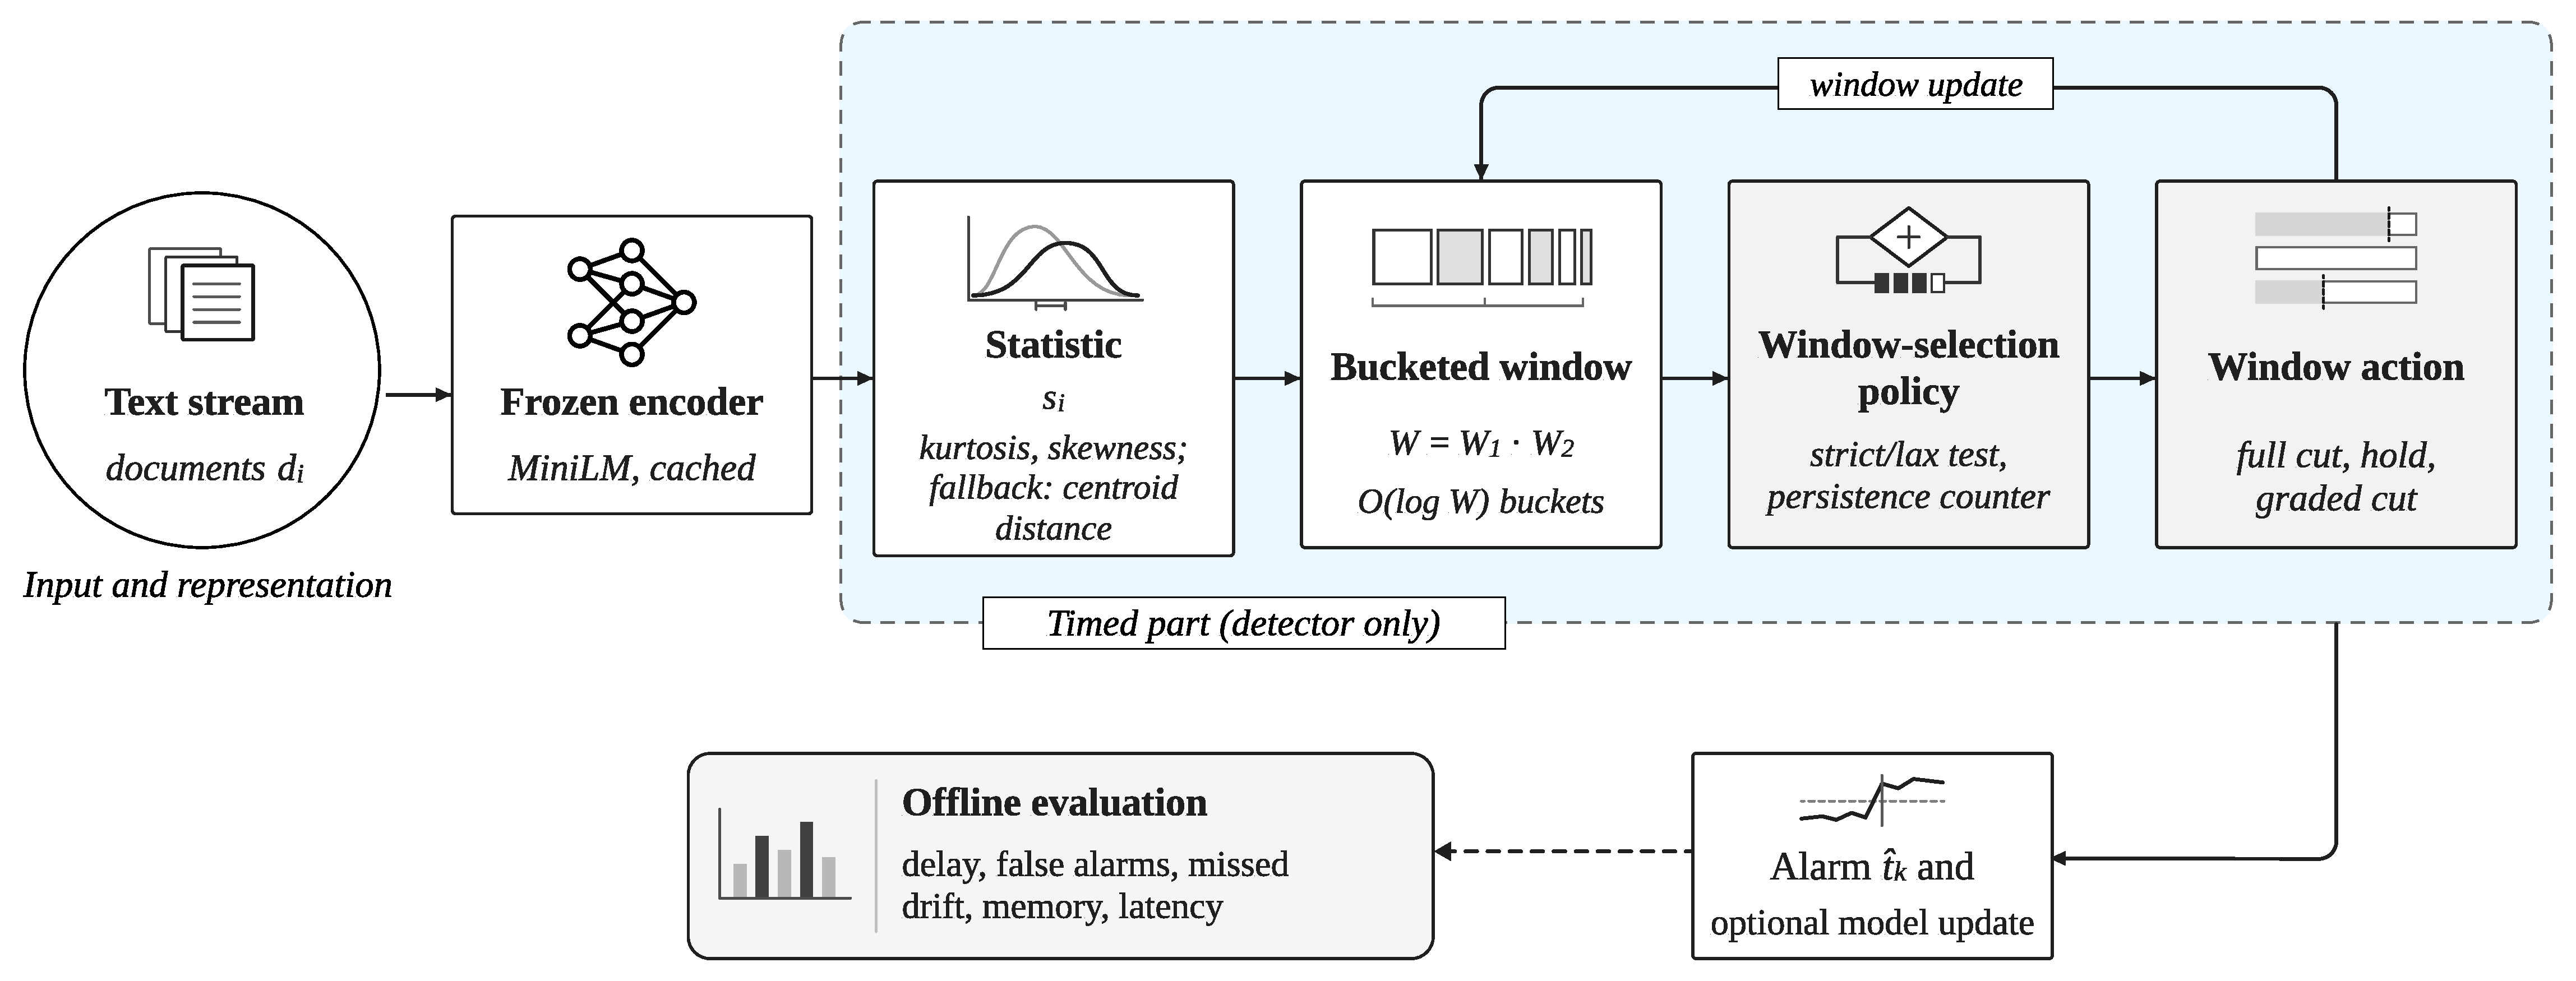
\includegraphics[width=0.98\linewidth]{figures/pipeline.pdf}
\end{center}

\begin{itemize}
  \item \textbf{What it shows:} the full path from a document to an alarm. The shaded box (window-selection policy) is our new part.
  \item \textbf{How to read it (left to right):} \emph{Text stream} $\to$ \emph{Frozen encoder} (MiniLM, cached) $\to$ \emph{Statistic} (kurtosis or skewness, with the centroid distance as backup) $\to$ \emph{Bucketed window} ($W=W_1\cdot W_2$, $O(\log W)$ buckets) $\to$ \emph{Window-selection policy} (strict and lax test, persistence counter) $\to$ \emph{Window action} (full cut, hold, graded cut). The top arrow ``window update'' sends the result back to the window. The action then gives an \emph{alarm} and an optional model update.
  \item \textbf{Other parts of the figure:} the bracket ``Timed part (detector only)'' shows what we time, and the \emph{Offline evaluation} box lists what we measure (delay, false alarms, missed drift, memory, latency).
  \item \textbf{Why we added it:} so a reader sees the whole system in one look and sees exactly \emph{where} our work fits. Everything before the shaded box is taken from existing work. Only the policy is new.
  \item \textbf{Key point to say:} the embeddings are cached, so the timing we report covers only the detector and not the encoder.
\end{itemize}

\subsection{Figure 2: State diagram of the policy}

\begin{center}
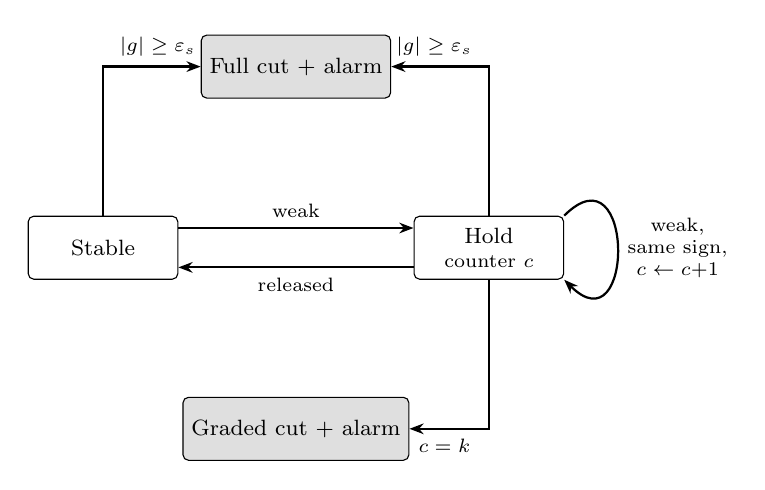
\begin{tikzpicture}[
  st/.style={draw, rounded corners=2pt, align=center, minimum height=8mm, minimum width=1.9cm, inner sep=3pt, font=\footnotesize, fill=white},
  ac/.style={draw, rounded corners=2pt, align=center, minimum height=8mm, inner sep=3pt, font=\footnotesize, fill=gray!25},
  arr/.style={-{Stealth[length=1.8mm]}, thick},
  lab/.style={font=\scriptsize, align=center}
]
\node[st] (stable) at (0,0) {Stable};
\node[st] (hold) at (4.9,0) {Hold\\[-1pt]{\scriptsize counter $c$}};
\node[ac] (full) at (2.45,2.3) {Full cut + alarm};
\node[ac] (grad) at (2.45,-2.3) {Graded cut + alarm};
\draw[arr] (stable.north) |- node[lab, pos=0.78, above] {$|g|\ge\varepsilon_s$} (full.west);
\draw[arr] (hold.north) |- node[lab, pos=0.78, above] {$|g|\ge\varepsilon_s$} (full.east);
\draw[arr] ([yshift=2.5mm]stable.east) -- node[lab, above] {weak} ([yshift=2.5mm]hold.west);
\draw[arr] ([yshift=-2.5mm]hold.west) -- node[lab, below] {released} ([yshift=-2.5mm]stable.east);
\draw[arr] (hold.south) |- node[lab, pos=0.78, below] {$c=k$} (grad.east);
\draw[arr] (hold.north east) .. controls +(0.9,0.9) and +(0.9,-0.9) .. node[lab, right, pos=0.5] {weak,\\same sign,\\$c\leftarrow c{+}1$} (hold.south east);
\end{tikzpicture}
\end{center}

\begin{itemize}
  \item \textbf{What it shows:} the states of the policy and the rules to move between them. White boxes are states where we watch. Grey boxes are actions where the window is cut.
  \item \textbf{How to read it (follow the arrows):}
  \begin{itemize}
    \item From \textbf{Stable}, a strong gap ($|g|\ge\varepsilon_s$) goes straight to a \textbf{full cut}.
    \item From \textbf{Stable}, a weak gap goes to \textbf{Hold}.
    \item In \textbf{Hold}, if the weak gap continues with the same sign, the loop arrow adds one to the counter $c$.
    \item In \textbf{Hold}, if the gap becomes strong, we do a full cut. If the gap vanishes or changes sign, it is \emph{released} back to Stable. If $c=k$, we do a \textbf{graded cut}.
    \item After any cut, the policy goes back to Stable.
  \end{itemize}
  \item \textbf{Why we added it:} the policy has several rules, and a picture is easier to follow than a paragraph. It also proves that every case has a defined action.
\end{itemize}

\subsection{Figure 3: Full cut compared with graded cut}

\begin{center}
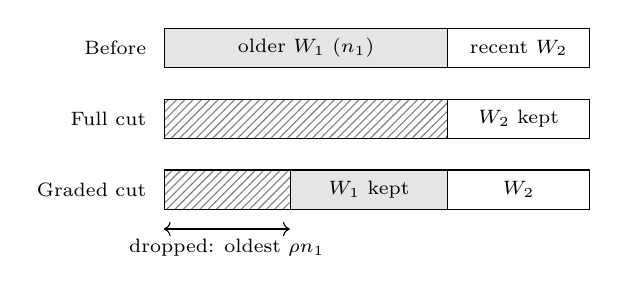
\begin{tikzpicture}[
  seg/.style={draw, minimum height=5mm, inner sep=0pt, font=\scriptsize},
  lab/.style={font=\scriptsize, anchor=east}
]
\def\a{3.6} \def\b{1.8} \def\d{1.6} \pgfmathsetmacro{\r}{\a-\d}
\node[lab] at (0,0) {Before};
\node[seg, minimum width=\a cm, fill=gray!20, anchor=west] (a1) at (0.1,0) {older $W_1$ ($n_1$)};
\node[seg, minimum width=\b cm, fill=white, anchor=west] (a2) at (\a+0.1,0) {recent $W_2$};
\node[lab] at (0,-0.9) {Full cut};
\node[seg, minimum width=\a cm, pattern=north east lines, pattern color=black!50, anchor=west] at (0.1,-0.9) {};
\node[seg, minimum width=\b cm, fill=white, anchor=west] at (\a+0.1,-0.9) {$W_2$ kept};
\node[lab] at (0,-1.8) {Graded cut};
\node[seg, minimum width=\d cm, pattern=north east lines, pattern color=black!50, anchor=west] at (0.1,-1.8) {};
\node[seg, minimum width=\r cm, fill=gray!20, anchor=west] at (\d+0.1,-1.8) {$W_1$ kept};
\node[seg, minimum width=\b cm, fill=white, anchor=west] at (\a+0.1,-1.8) {$W_2$};
\draw[<->, thin] (0.1,-2.3) -- node[font=\scriptsize, below] {dropped: oldest $\rho n_1$} (\d+0.1,-2.3);
\end{tikzpicture}
\end{center}

\begin{itemize}
  \item \textbf{What it shows:} the window as a bar. The left side is old data ($W_1$) and the right side is recent data ($W_2$). Hatched (striped) parts are the data that were dropped.
  \item \textbf{How to read it:} the top row is the window before any cut. In the \emph{full cut} row, all of $W_1$ is dropped and only $W_2$ remains. In the \emph{graded cut} row, only the oldest part of $W_1$ is dropped (the length is $\rho\, n_1$) and the rest of $W_1$ stays.
  \item \textbf{Why we added it:} it is the most important difference from ADWIN-U. ADWIN-U always does the middle row. Our policy can do the bottom row, so it keeps useful older data when the change is only small. More data means a steadier estimate.
\end{itemize}

\subsection{Table I: Planned datasets}
The table lists the three datasets, the role of each and whether the drift points are known. We added it because it shows in one place that our evaluation has both controlled streams (known drift, so we can measure delay exactly) and a real stream (unknown drift, so we test in real conditions).

%====================================================================
\section{Evaluation Plan Explained}

\subsection{Datasets}

\begin{center}
\small
\begin{tabular}{@{}>{\bfseries}p{2.8cm}p{7.6cm}p{2.4cm}@{}}
\toprule
Dataset & How we use it & Drift points \\
\midrule
AG News & We change the topic mix to build drift: a single switch (abrupt), a smooth sigmoid change (gradual), and a return to an earlier mix (recurring). & Known \\
20 Newsgroups & Swapping groups from different macro-topics gives strong drift. Swapping sibling groups gives subtle drift. & Known \\
Amazon reviews & A real stream of timestamped reviews in time order. We use proxies such as the alarm rate, downstream accuracy for a given label budget, and alignment with a known event. & Unknown \\
\bottomrule
\end{tabular}
\end{center}

\textbf{Why these three?} They cover different kinds of text (news, discussion posts and reviews). They also cover different levels of certainty, from known injected drift to unknown real drift. This links to \emph{variety} and \emph{veracity}.

\subsection{Baselines (what we compare with)}
\begin{itemize}
  \item \textbf{ADWIN-U} (single and multiple detectors): our base paper.
  \item \textbf{Plain ADWIN with a grid of $\delta$ values:} tests whether our gain is only because of tuning $\delta$.
  \item \textbf{Two-threshold warning/alarm variant:} tests whether the gain comes only from adding a warning zone.
  \item \textbf{KSWIN-style test:} a fixed-window method with the Kolmogorov--Smirnov test.
  \item \textbf{D3-style detector:} trains a classifier to tell old from new data and watches its AUC.
\end{itemize}

\subsection{Metrics (how we measure)}
\begin{center}
\small
\begin{tabular}{@{}>{\bfseries}p{4.3cm}p{9cm}@{}}
\toprule
Metric & Easy meaning \\
\midrule
Mean time to detection & How many items pass between the real drift and our alarm. Smaller is better. \\
False alarms per 1,000 & Alarms when nothing changed. Smaller is better. \\
Missed-drift rate & Share of real drifts we never detected. Smaller is better. \\
Window length & How long the window stays. Shows how much data we keep. \\
Per-instance latency & Time to process one item. Shows speed (velocity). \\
Peak memory & The most memory used. Shows if it is light enough. \\
Throughput & Documents handled per second. Shows if we keep up with the stream. \\
BAR (secondary) & A score from the base paper that combines accuracy with the share of labels requested. We use it only as extra evidence. \\
\bottomrule
\end{tabular}
\end{center}

\textbf{Why not use accuracy as the main score?} Lukats et al.\ showed that accuracy-based scores can favor detectors that fire very often, because frequent updates keep the model fresh. So we measure delay and false alarms directly.

\subsection{Fair testing}
\begin{enumerate}
  \item First, we set all detectors to the \textbf{same false-alarm rate} on a stream with no drift. Then no detector wins just by being more sensitive.
  \item We test on \textbf{several random stream orders} and rank the detectors with the \textbf{Friedman and Nemenyi tests}. These are standard tests to compare many methods over many datasets.
  \item \textbf{Ablations:} we turn off parts of our method (hold only, graded cut without persistence, full policy) to see which part helps the most.
\end{enumerate}

%====================================================================
\section{Literature Review in Short}

\begin{center}
\small
\begin{tabular}{@{}>{\bfseries}p{3.1cm}p{5.2cm}p{4.9cm}@{}}
\toprule
Group & Main works in our report & What we take from it \\
\midrule
Drift surveys & Gama et al.\ 2014; Lu et al.\ 2019; Webb et al.\ 2016 & Definitions and types of drift. \\
Supervised detectors & DDM (Gama 2004); ADWIN (Bifet 2007) & They need labels, which is our problem. \\
Unsupervised detectors & Hinder et al.\ 2024; KSWIN (Raab 2020); D3 (G\"oz\"ua\c{c}\i k 2019); Lukats et al.\ 2025 & Window comparison idea and our baselines. \\
Window methods & DAWIDD; Chen et al.\ 2024; Klinkenberg and Joachims 2000; Kuncheva and \v{Z}liobait\.{e} 2009 & Other ways to choose windows. Most need labels or a classifier. \\
Applied systems & Mehmood 2024; Badar 2023; Hu 2024 & Window handling in real systems. None gives a general label-free policy for how much to drop. \\
Base paper & ADWIN-U (Assis and Souza 2025) & Label-free adaptive window. \\
Text streams & Garcia et al.\ 2025; Sentence-BERT (Reimers 2019) & Few text benchmarks. Text is turned into vectors with encoders. \\
\bottomrule
\end{tabular}
\end{center}

\textbf{Summary to say:} Window choice shapes what a detector sees. ADWIN-U gives a label-free adaptive window. Text streams lack a tested evaluation protocol. What is missing is a rule that uses the strength and persistence of the evidence to decide how the window changes, together with a test on text. This is exactly our contribution.

%====================================================================
\section{Where Are We Now? (Honest Status)}

\begin{itemize}
  \item \textbf{Done:} problem definition, literature review, base paper study, research gap, the policy design, figures and the evaluation plan.
  \item \textbf{Not done yet:} experiments and results. The report is an idea and plan, as the faculty asked for the midterm.
  \item \textbf{Next steps:} build the text streams, implement the policy on top of ADWIN-U, run the baselines at the same false-alarm rate, and report the metrics.
  \item \textbf{Expected, not proven:} the policy should give a better balance of delay, false alarms and missed drift, especially for gradual and subtle drift. We will confirm this only with experiments.
\end{itemize}

%====================================================================
\section{Possible Questions and Short Answers}
\label{sec:qa}

\begin{description}[style=nextline,leftmargin=0.5cm]
\item[Q1. What is the main problem you solve?]
Drift detectors need labels, but labels are late or missing in text streams. ADWIN-U works without labels, but it cuts the window in an all-or-nothing way. We improve this cut rule and test it on text.

\item[Q2. What is your base paper?]
ADWIN-U by Assis and Souza (Knowledge and Information Systems, 2025). It builds on ADWIN by Bifet and Gavald\`a (2007).

\item[Q3. What exactly is new in your work?]
A policy with two thresholds, a hold state, a counter for persistence and a partial cut whose size depends on the gap. ADWIN-U is a special case. We also test on text, which the base paper did not.

\item[Q4. Are you claiming you invented adaptive windows?]
No. ADWIN and ADWIN-U already provide the window and label-free monitoring. Our contribution is the rule for \emph{how the window changes}, and its evaluation on text.

\item[Q5. Why text streams?]
Text changes often (new events, new words), and labels are expensive. So label-free detection is very useful. Also, ADWIN-U was tested only on numeric data.

\item[Q6. How do you work with text if the detector needs numbers?]
We use a frozen Sentence-BERT model to turn each document into a 384-number embedding. Then we compute one statistic (skewness or kurtosis) per embedding.

\item[Q7. What if skewness or kurtosis does not detect topic changes?]
This is a real risk, and we say so in the report. We test it first. As a backup we use the cosine distance between each embedding and the window centroid.

\item[Q8. Why do you need a hold state?]
A single weak signal may be noise. The hold waits to see if the signal lasts in the same direction. This reduces false alarms and still catches slow drift.

\item[Q9. Will the hold state delay detection?]
For strong changes, no, because a full cut happens at once. For weak changes, the hold waits $k$ checks, but ADWIN-U may not detect them at all. The value of $k$ will be tuned and tested in ablations.

\item[Q10. Does your method give a guarantee on false alarms?]
Not fully. The strict bound has a guarantee, but the relaxed test with persistence does not. That is why we measure false alarms on streams with no drift and compare at the same false-alarm rate.

\item[Q11. Is it fast enough for real-time use?]
We expect the cost to stay close to ADWIN-U's $O(\log W)$, since we add only a counter and a sign. We will measure latency, throughput and peak memory.

\item[Q12. Where are your results?]
This is a midterm report with the idea and the plan. Experiments come next. We describe the datasets, baselines, metrics and tests we will use.

\item[Q13. Which big data characteristics do you cover?]
Velocity (one-pass, compact window, low latency), Variety (unstructured text of different topics and styles) and Veracity (no labels, unknown drift points, and no action on a single weak signal). We do not claim Volume.

\item[Q14. How do you know that a gain comes from your policy and not from tuning?]
We compare with plain ADWIN on a grid of $\delta$ values and with a warning/alarm variant. We set all methods to the same false-alarm rate and run ablations.

\item[Q15. How do you test on the Amazon stream if the drift points are unknown?]
We use proxies: the alarm rate, downstream accuracy for a given label budget, and alignment with a known event. We are careful to call these proxies and not proof.

\item[Q16. Why only these references?]
We use only published journal and conference papers, not preprints, so that the sources are reliable.
\end{description}

%====================================================================
\section{Simple Words List (Glossary)}

\begin{center}
\small
\begin{tabular}{@{}>{\bfseries}p{3.4cm}p{9.8cm}@{}}
\toprule
Word & Easy meaning \\
\midrule
Data stream & Data that keeps coming one item at a time, with no end. \\
Concept drift & The data changes over time, so an old model gets worse. \\
Unsupervised & Works without the true labels. \\
Window & The recent part of the stream that we keep in memory. \\
$W_1$, $W_2$ & The older part and the newer part of the window. \\
ADWIN & A method that keeps a window of variable length and cuts the old part when a change is found. \\
ADWIN-U & ADWIN made to work without labels, by watching a statistic of the data. \\
Statistic & One number that describes data, like the mean, skewness or kurtosis. \\
Embedding & A list of numbers that stands for the meaning of a text. \\
Sentence-BERT & A pre-trained model that makes embeddings from sentences. \\
Frozen model & A model we use as it is, without training it again. \\
Threshold ($\varepsilon$) & The size of the gap above which we say ``this is a real change''. \\
Confidence level ($\delta$) & A small number that controls how strict the test is. Smaller means stricter. \\
Hoeffding bound & A math result that says how far an average can move by pure chance. \\
False alarm & The detector says ``drift'' but nothing changed. \\
Missed drift & A real drift that the detector never reports. \\
Detection delay & The time from the real drift until the alarm. \\
Hold state & A waiting state: we saw weak evidence and do not cut yet. \\
Graded cut & Dropping only a part of the old window, based on the gap size. \\
Ablation & A test where we remove one part of our method to see how much it matters. \\
Baseline & Another method we compare with. \\
Throughput & How many documents we process per second. \\
\bottomrule
\end{tabular}
\end{center}

%====================================================================
\section{Suggested Talking Order for the Class}

\begin{enumerate}
  \item \textbf{Problem} (1 min): text changes, labels are missing, models get old.
  \item \textbf{Background} (1 min): concept drift, window size trade-off.
  \item \textbf{Base paper and gap} (2 min): ADWIN-U, the all-or-nothing cut, no text tests.
  \item \textbf{Our idea} (2 min): two thresholds, hold, graded cut. Use Figures 2 and 3.
  \item \textbf{Pipeline} (1 min): use Figure 1 and say why embeddings are cached.
  \item \textbf{Evaluation plan} (1 min): datasets, baselines, metrics, fair testing.
  \item \textbf{Big data link} (1 min): velocity, variety and veracity.
  \item \textbf{Status and next steps} (1 min): idea and plan done, experiments next.
\end{enumerate}

\end{document}
